\documentclass[10pt,fleqn]{article}
\usepackage{/home/clair/Documents/mystyle}

\usetikzlibrary{automata, positioning, shapes.multipart, arrows}

%----------------------------------------------------------------------
% reformat section headers to be smaller \& left-aligned
\titleformat{\section}
	{\normalfont\bfseries}
	{\thesection}{1em}{}
	
\titleformat{\subsection}
	{\normalfont\bfseries}
	{\thesubsection}{1em}{}

%======================================================================
\newcommand{\q}[1]{
	\begin{minipage}{\textwidth}
	\textcolor{black}{
					\begin{tabular}{p{0.01\textwidth}p{0.95\textwidth}}
						$\square$ & #1
					\end{tabular}
					}
	\end{minipage}
}

%======================================================================

\begin{document}

\section*{QUESTIONS / CONSIDERATIONS / CHANGES TO CLASSIFICATIONS}

\q{Perhaps distinguish between hot pixels (those that are bright in black image) and bright pixels (those that become bright when hit with an xray source)? Would then be a qualitative difference, rather than quantitative.} 

\q{Likewise, make qualitative distinction among pixels with lower-than-normal response: dim pixels have lower-than-expected value (possibly also in the black image?) but no-response pixels don't show any activity when exposed to x-ray source}

\q{Screen spots are not relevant for the state space problem, so will be treated as part of the healthy pixel population. However, we should still identify them, to avoid wrongly classifying those groups of pixels as individually defective.}

\q{When compiling Markov model, treat non-responsive/dead columns, such as those seen in the old data, as censored individuals.  We don't know what state they are in because their charge is blocked.}

\q{For pixels on a bright line - could treat all pixels along line as a separate group (on the assumption that `bright line' behaviour will subsume individual pixel behaviour) or adjust by observed column offset \& reclassify? according to new values? Propose treating pixels along the affected column like any other pixel, since increased current is not occuring in the pixels themselves, but in readout. However, pixel at root of line (end furthest from panel edge) should be classified differently}

\q{How to handle clusters/hot pixel `bleeds'? In a sense, nothing has gone wrong with the pixels on the edge, they're being affected by an external factor (neighbouring hot pixel), just like the lines. Proposed solution: set cluster midpoint (or brightest point - this may be more consistent) to `cluster' type, then censor all other pixels in that cluster.}

\q{Also still considering whether to allow misclassification between states (eg. could a hot pixel sometimes appear only bright?). Will investigate once the standard model is up and running...}

\newpage

\section{Glossary of defective pixel types}

\begin{footnotesize}
\begin{description}
\item[Locally bright:] pixelwise mean value is greater than the median of its neighbours by more than 2$\times$ the image's MAD

\item[Bright:] currently anything above (median + 0.25 $\times$ (max - median)) at any power setting. \emph{\textcolor{blue}{Possible alternative: anything above this limit in grey/white images (ie. with x-ray source) only}}

\item[Hot:] currently any pixel that reaches maximum value of 65535 in the black images. \emph{\textcolor{blue}{Possible alternative: use same threshold calculation as for bright pixels, but for black images only (ie. only include pixels that are bright without any x-ray encouragement)}}

\item[Locally dim:] pixelwise mean value is lower than the median of its neighbours by more than 2$\times$ the image's MAD

\item[Dim:] anything below (median - 0.25 $\times$ (median - min)) at any power setting, excluding pixels already identified as non-responsive. (Includes the 3 dead pixels, which form a single non-communicating class in the available data)

\item[No response:] Pixel behaves normally in black images, but response in grey/white images remains at normal black level. No response at all to presence of x-rays.

\item[Cluster:] A group of between 2 and 9 adjacent defective pixels of any type. Can be divided into those containing a non-responsive pixel (or pixels) and those containing a hot pixel (or pixels). \emph{\textcolor{blue}{Propose labelling only the brightest/darkest pixel as the `root', and the other cluster elements as censored}}

\item[Line root:] The defective pixel at the `free' end of a line (that is, the end that doesn't reach the midline/panel edge, depending on the type of line).

\item[Blocked:] Any pixel covered by a cluster or line, which is not the `root' of the feature. Treated as a censored individual in model fitting, since it is no longer functioning as an independent pixel.

\end{description}
\end{footnotesize}

\section{State spaces observed in a single acquisition}

%\href{http://tex.stackexchange.com/questions/178904/use-datatool-to-read-a-row-from-a-csv-file-then-use-the-variables-in-the-docume}{Read data into variables using \texttt{datatool}} \\
%\href{http://www.texample.net/tikz/examples/state-machine/}{State machine in \texttt{tikz}}

\begin{figure}[!h]
\caption{Current working state space model for individual pixels.}

\tikzstyle{state}=[rectangle, draw=black, rounded corners, text centered, anchor=north, text width=2cm, minimum height = 1.5cm]
        
 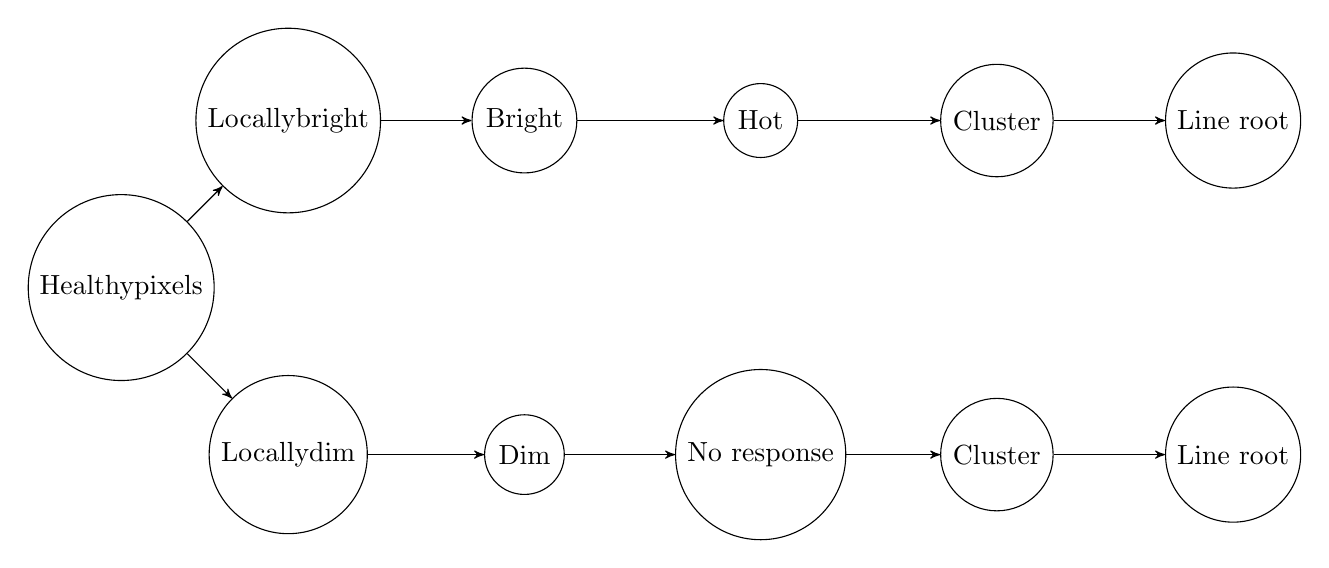
\begin{tikzpicture}[node distance=3cm,on grid,auto,>=stealth'] 

% State nodes
	\node (healthy)		[state]		{Healthy \\ pixels};	

	\node (loc_dim)		[state, below right=of healthy]		{Locally \\ dim};
	\node (dim)			[state, right=of loc_dim]			{Dim};
    \node (no_resp)		[state, right=of dim] 				{No response}; 
	\node (dark_clust)	[state, right=of no_resp]			{Cluster};
	\node (dark_root)	[state, right=of dark_clust]			{Line root}; 
    
    \node (loc_bright)	[state, above right = of healthy]	{Locally \\ bright};
    \node (bright)		[state, right = of loc_bright]		{Bright};
    \node (hot)			[state, right = of bright]			{Hot};
    \node (hot_clust)	[state, right = of hot]				{Cluster};
    \node (hot_root)		[state, right = of hot_clust]		{Line root};



% Add column & row headers
	\path[->] 
		(healthy)		edge	 node {} (loc_dim)
		(healthy)		edge	 node {} (loc_bright)

		(loc_dim)		edge	 node {} (dim)
		(dim)			edge	 node {} (no_resp)
		(no_resp)		edge	 node {} (dark_clust)
		(dark_clust)		edge	 node {} (dark_root)
		
		(loc_bright)		edge node {} (bright)
		(bright)			edge node {} (hot)
		(hot)			edge node {} (hot_clust)
		(hot_clust)		edge node {} (hot_root)
	;

\end{tikzpicture}
\end{figure}

\subsection{Stability of rate changes: constant or increasing? (Or decreasing, even?)}

\q{Plot number of pixels identified as each type of bad over all 12 acquisitions: is trend linear?}

\section{Still to do}

\q{Plot each threshold (in terms of $\sigma$ vs \% of problematic pixels identified}

\q{Relate each type of bad pixel to behaviour in shading correction: may suggest adjustments to thresholds}

\q{Tabulate best-case vs worst-case scenario for classification (essentially, switching sort order before removing duplicates)}

%\newpage
%\printbibliography
\end{document}
